\section{Статья 2: Исследование генетических операторов в программировании с экспрессией генов}

\subsection{Введение}

В ПЭГ применяются следующие операторы: репликации, мутации, копирования со сдвигом, копирования со двигом в корень, перестановки генов, одно- и двухточечной рекомбинации, генной рекомбинации. Рассмотрим каждый из них.

Репликация представляет собой самый простой оператор, не вносящий разнообразие в геном. Используется в паре с оператором отбора для копирования особей в новую популяцию в соответствии со значением фитнеса и случайностью, вводимой оператором рулетки.

Мутация (замена символа~--- элемента гена, соответствующего узлу дерева) может возникнуть в любом месте хромосомы. Вероятность оператора, как правило, задаётся эквивалентной двум мутациям в хромосоме. Элементы, подвергающиеся мутации в голове гена, могут быть изменены на любой другой символ (функцию или терминал), в хвосте~--- только на терминал. Данное ограничение нацелено на сохранение структуры хромосомы и обеспечение декодирования синтаксически верного дерева. Среди всех модифицирующих операторов мутация является самым важным и эффективным, т.к. в отличие от остальных, комбинирующих существующие участки генома, мутация направлена на создание новых элементов, а потому вносит наиболее радикальные изменения, расширяя область поиска решений.

В ходе анализа существующих методов и средств, направленных на ускорение получения модели алгоритмом ПЭГ и повышение её качества, а также проведённых экспериментов был выявлен ряд ограничений производительности алгоритма, таких как длительность вычисления фитнеса, отсутствие тонкой подстройки числовых констант, вляние размера хромосомы на скорость сходимости, проблемы с поиском сложных моделей. Далее описаны методы и подходы, созданные в ходе преодоления данных ограничений.

Алгоритм ПЭГ заключается в выполнении следующих этапов:
\begin{enumerate} \itemsep0pt \parskip0pt \parsep0pt
  \item Создание начальной популяции
  \item Декодирование особей
  \item Выполнение программ особей
  \item Вычисление фитнеса особей
  \item Проверка критерия останова алгоритма (достигнута требуемая точность, либо истекло лимитированное время выполнения)
  \item Копирование лучшей особи (Элитизм)
  \item Отбор
  \item Репликация
  \item Мутация
  \item Операторы переноса
  \item Операторы рекомбинации
  \item Возврат к пункту 2
\end{enumerate}


%--------------------------------------------------------------------


\subsection{Методика тестирования}

В предыдущей статье цикла [ссылка на статью 1] описана методика оценки эффективности модификаций алгоритма ПЭГ, заключающаяся в статистической обработке результатов множества запусков с целью получения таких основных метрик: СКО наилучшей модели среди всех запусков ($e_{b}$) и доля успешных запусков ($r_{f}$)~--- таких, в ходе которых была получена модель с приемлемой для данной задачи точностью.

Тестирование производилось на следующих задачах:
\begin{enumerate}
  \item $y(x) = \sin x, x \in [-5, 4.6]$;
  \item Функция Розенброка: $z(x, y) = {(1 - x)}^2 + 100 {(y - x^2)}^2, x \in [-3, 3], y \in [-3, 3]$;
  \item Сумма четырёх сигмоид:
    \begin{multline}
      z(x, y) = \frac{1}{2} \times \exp\left(-\frac{(9x-2)^2 - (9y-2)^2}{4}\right) + \frac{3}{4} \times \exp\left(-\frac{(9x+1)^2}{49} + \frac{(9y+1)^2}{10}\right) + \\
      + \frac{1}{2} \times \exp\left(-\cfrac{(9x-7)^2 + (9y-3)^2}{4}\right) -\frac{1}{5} \times \exp\left(-(9x-4)^2 - (9y-7)^2\right), \\
      x \in [-2, 2], y \in [-2, 2]
    \end{multline}
\end{enumerate}



%--------------------------------------------------------------------



\subsection{Операторы отбора}

Процесс эволюции основан на генетической изменчивости и процедуре отбора. Эти же механизмы задействованы во всех эволюционных алгоритмах. Однако способ обеспечения генетической изменчивости, который можно было бы назвать лучшим, не был выявлен. Исследователи разделяют эти способы на мутацию и рекомбинацию. Успешность эволюции также сильно зависит от применяемых алгоритмом генетических операторов, размера и состава начальной популяции.

Сравнивая эффективность исходного алгоритма ПЭГ при разных размерах популяции следует учесть, что время выполнения алгоритма прямо пропорционально размеру популяции. Для оценки данного фактора в условиях ограниченного времени время каждому запуску было отведено фиксированное время работы, потому алгоритмы с б\'{о}льшим размером популяции имели возможность расчитать меньшее число поколений. Результаты продемонстрированы в таблице~\ref{tbl:cmp_pop_sizes}, из которых также следует наличие пика эффективности при размере популяции 80--120~особей.

\input{cmp_pop_sizes}

Одно из важнейших применений ПЭГ~--- символьная регрессия, цель которой~--- поиск выражения, наиболее соответствующего известным заданным значениям с определённой погрешностью. Установка небольшого значения (абсолютного или относительного) этой погрешности позволит обнаружить хорошие решения некоторых математических задач, однако в большинстве случаев маленькая допустимая погрешность замедляет эволюционирование по причине более строгого отбора особей. Если же задать слишком большую допустимую погрешность, отбор пройдёт множество особей, не являющихся приемлемыми решениями, однако значение фитнеса которых будет очень высоким.

Отбор особей в ПЭГ осуществляется пропорциональным оператором рулетки с простым элитизмом: лучшая особь популяции переносится в следующее поколение, шансы остальных прямо пропорциональны их фитнесу. Такая форма элитизма гарантирует, что лучшее обнаруженное решение не будет утрачено. Каждый запуск рулетки выбирает одну особь, соответственно, количество запусков рулетки равно размеру популяции.
После отбора новой популяции поочерёдно выполняются генетические операторы, применяемые к случайным образом выбранным особям. Например, если вероятность оператора составляет~70\%, то~7 из~10 особей будут им модифицированы. Каждая особь может быть модифицирована сразу несколькими операторами, однако оператор может быть применён к особи лишь однократно. Это отличает ПЭГ от~ГП, где особь не изменяется более чем одним оператором за итерацию. Получаемое таким образом потомство существенно отличается от родительских особей.

Наиболее универсальный оператор отбора с достаточной эффективностью, применяемый в ПЭГ~--- алгоритм рулетки, в котором вероятность дальнейшего участия особи в процессе эволюции напрямую определяется её фитнесом, что ведёт к сохранению только особей с высоким фитнесом. Однако если фитнес одной из особей популяции в определённый момент значительно превышает фитнес остальных, это приводит к застреванию алгоритма в локальном оптимуме и потере множества особей с тенденцией к улучшению, но небольшим текущим значением фитнеса.

В работе~\cite{conf/icnc/PengTZY05} предложена формула отбора, почерпнутая из иммунных алгоритмов, основанная на понятии плотности $D$ особи:

\begin{equation}
\label{eq:EAOGE_density}
D(I_k) = \frac{1}{\sum\limits_{i=1}^N{|f(I_k) - f(I_i)|}}, k=1,2,\ldots,N,
\end{equation}
где $N$~--- количество особей в популяции, $f$~--- функция фитнеса. Значения плотности используются затем для вычисления вероятности отбора:

\begin{equation}
\label{eq:EAOGE_probability}
P(I_k) = \frac{\sum\limits_{i=1}^N{D(I_k)}}{D(I_k)}, k=1,2,\ldots,N
\end{equation}

Таким образом, чем больше особей, похожих (по критерию вероятности) на особь $I_k$, тем меньшую вероятность отбора она имеет. Авторами не отмечается тот факт, что особи с принципиально разными синтаксическими деревьями, но равным значением фитнеса будут неотличимы друг от друга при данном подходе. Высказано предположение о том, что данная формула отбора гарантирует разнообразие генетического материала в популяции.

Сравнение различных подходов к механизму отбора предоставлено в таблице~\ref{tbl:cmp_probability_density_selection_and_tournament}. Во всех случаях осуществление простого элитизма осуществлялось путём сохранения лучшей особи. Анализ этих результатов позволяет сделать определённые выводы. Наиболее общим является целесообразность использования популяции размером в 50~особей: это экспериментально выведенное оптимальное значение характерно для всех девяти проведённых экспериментов. Исходный алгоритм ПЭГ (с кодированием путём обхода графа в ширину) достигает максимума своей производительности при использовании турнирного отбора. Для ПЭГ с наложениями таковым является отбор по плотности. Глобально же наилучшие результаты показывает префиксное ПЭГ в комбинации с оператором рулетки.

Таким образом, рассматривая операторы отбора вне зависимости от способа кодирования, наиболее оптимальным будет выбор оператора рулетки, как и было предложено автором оригинального алгоритма ПЭГ.

\input{cmp_probability_density_selection_and_tournament}



%--------------------------------------------------------------------



\subsection{Оператор мутации}

\subsubsection{Влияние на динамику эволюции}

В системах на основе генотипа и фенотипа пространство поиска отделено от пространства решений, что существенно улучшает производительность таких систем. Чем меньше ограничений накладывается на процедуру проецирования генотипа на фенотип и обратно~--- тем более эффективна система, т.к. практически любой оператор может быть использован для исследования пространства поиска, включая мутацию.

Так, например, в системе DGP (Developmental Genetic Programming~--- ГП с развитием~\cite{poli2008field}) в результате трансляции генотипа в фенотип не всегда получается синтаксически верное дерево, что приводит к необходимости проведения дополнительных операций по устранению непригодных особей. Потому мутация в DGP не превосходит по показателям операторы кроссовера.

Для сравнения эффективности каждого из генетических операторов, применяемых в ПЭГ, по отдельности были сопоставлены динамические данные процесса эволюции: графики фитнеса лучшей особи с течением поколений (итераций), и графики среднего фитнеса популяции~\cite{ferreira:2002:FEA}.

В ходе поиска модели, созданной формулой $y(x) = x^4 + x^3 + x^2 + x$ была исследована динамика эволюционного процесса с различными значениями вероятности применения оператора мутации ($p_{m_1}, p_{m_2}, p_{m_3}, p_{m_4}$), значения фитнеса приведены на рисунке~\ref{img:cmp_health}.

\begin{figure} [h]
  \center
  \begin{subfigure}[h]{0.3\linewidth}
    \center
    \begin{tikzpicture}
      \begin{axis}[title={а) $p_{m_1} = 0$}, width=\linewidth, no marks, ymax = 1000, ylabel={Фитнес}, xlabel={Время, мс}, legend entries={{Лучший фитнес},{Средний фитнес}}, legend to name=legend_local_refcmp_health, legend columns=2]
        \addplot[mark=x,red] table[x=time,y=best] {data_health_0};
        \addplot[mark=*,blue] table[x=time,y=mean] {data_health_0};
      \end{axis}
    \end{tikzpicture}
  \end{subfigure}
  \begin{subfigure}[h]{0.3\linewidth}
    \center
    \begin{tikzpicture}
      \begin{axis}[title={б) $p_{m_2} > p_{m_1}$}, width=\linewidth, no marks, ymax = 1000, ylabel={Фитнес}, xlabel={Время, мс}]
        \addplot[mark=x,red] table[x=time,y=best] {data_health_1};
        \addplot[mark=*,blue] table[x=time,y=mean] {data_health_1};
      \end{axis}
    \end{tikzpicture}
  \end{subfigure}
  \\
  \begin{subfigure}[h]{0.3\linewidth}
    \center
    \begin{tikzpicture}
      \begin{axis}[title={в) $p_{m_3} > p_{m_2}$}, width=\linewidth, no marks, ymax = 1000, ylabel={Фитнес}, xlabel={Время, мс}]
        \addplot[mark=x,red] table[x=time,y=best] {data_health_2};
        \addplot[mark=*,blue] table[x=time,y=mean] {data_health_2};
      \end{axis}
    \end{tikzpicture}
  \end{subfigure}
  \begin{subfigure}[h]{0.3\linewidth}
    \center
    \begin{tikzpicture}
      \begin{axis}[title={г) $p_{m_4} > p_{m_3}$}, width=\linewidth, no marks, ymax = 1000, ylabel={Фитнес}, xlabel={Время, мс}]
        \addplot[mark=x,red] table[x=time,y=best] {data_health_3};
        \addplot[mark=*,blue] table[x=time,y=mean] {data_health_3};
      \end{axis}
    \end{tikzpicture}
  \end{subfigure}
  \\
  \ref{legend_local_refcmp_health}
  \caption{Динамика эволюции при разных вероятностях мутации}
  \label{img:cmp_health}
\end{figure}

На рисунке~\ref{img:cmp_health}а видно, что график лучшего фитнеса практически совпадает с графиком среднего фитнеса, особенно в поздних поколениях. Такие популяции называются умеренно инновационными в силу небольшого разнообразия между особями и медленного процесса эволюции. Вероятность успешного обнаружения решения задачи, поставленной в эксперименте, составила~16\% (отношение запусков, в ходе которых решение было обнаружено, к общему количеству запусков алгоритма).

На следующем рисунке заметно, что форма графиков совпадает (не принимая во внимание колебания графика среднего фитнеса), однако они не пересекаются, между ними наблюдается разрыв. Процентное соотношение успешных запусков составило~47\%. Такая модель эволюции является здоровой, но слабой.

С повышением вероятности мутации возрастает успешность алгоритма, достигая максимума при $p_{m_3}=0.1$, показанного на рисунке~\ref{img:cmp_health}в: здоровая и сильная модель. Характерен б\'{о}льший разрыв между графиками, чем в предыдущем случае, однако с сохранением тенденции к росту среднего фитнеса.

Наконец, последняя приведённая динамика со средним фитнесом на постоянном низком уровне с небольшими колебаниями является примером полностью хаотической системы, в которой, несмотря на элитизм, каждое поколение является по сути случайным.

Исследование операторов рекомбинации в качестве единственных источников, вносящих генетическое разнообразие, выявило процесс усреднения популяции~--- быстрое сокращение разрыва между графиками лучшего и среднего фитнеса с последующим их перекрытием. Это означает, что геном всех особей популяции совпадает, и разнообразие устранено, что является следствием преждевременной сходимости такого подхода к локальному оптимуму.

В начальной популяции, заполненной особями, созданными случайным образом, жизнеспособные решения~--- событие редкое, особенно при решении сложных задач. Удачным подходом в таком случае будет начало процесса эволюции с одной или нескольких особей-основателей~\cite{HreFer02}. Эффект основателя, описанный Э.~Майром, как создание новой популяции из особей-основателей, может быть инициирован дрейфом генов~--- изменением частоты вариантов генов вследствие случайных процессов и работы операторов отбора. Наиболее выраженный случай эффекта основателя~--- колонизация необитаемой области (создание новой популяции) одной особью.

Это означает, что при определённом значении вероятности мутации можно добиться максимальной эффективности работы всего алгоритма. Кроме того, оператор мутации уменьшает тенденцию популяции к гомогенизации (утрате разнообразия), и устраняет сильную зависимость эффективности алгоритма от размера популяции.

%--------------------------------------------------------------------

\subsubsection{Влияние на производительность}

Влияние наиболее вероятных значений среднего количества мутаций на хромосому на работу алгоритмов с различными способами кодирования синтаксических деревьев показано в таблице~\ref{tbl:cmp_mutation_probabilites}. Отметим общий для всех способов кодирования максимум эффективности при 1--2~мутациях на хромосому. В случае ПЭГ с наложениями максимум эффективости выделить значительно сложнее, однако всё же прослеживается падение производительности при количестве мутаций более~2. В дальнейшем будет использоваться значение в 2~мутации.

\input{cmp_mutation_probabilites}

%--------------------------------------------------------------------

\subsubsection{Модификации}

Наибольшим недостатком алгоритма ПЭГ является его склонность к преждевременной сходимости к локальному оптимуму, потому любые техники, направленные на решение этой проблемы, приводят к существенному росту производительности ПЭГ, что выражается в сокращении времени сходимости, улучшении средней приспособленности решений, повышению вероятности успешного обнаружения оптимального решения.

Для усиления способности алгоритма к поиску предлагается~\cite{2008acat.confE.66T} следующий алгоритм динамической мутации DM-GEP. При максимальном количестве поколений $T$ процесс эволюции разбивается на три фазы:
\begin{enumerate} \itemsep0pt \parskip0pt \parsep0pt
  \item Начальная фаза: поколения от первого до $T_1$, $0 < T_1 < T$. Вероятность мутации $p_m$ возрастает каждые два поколения со значения 0.022 до 0.44 с шагом 0.001.
  \item Метафаза: поколения от $T_1$ до $T_2$, $T_1 < T_2 < T$. Вероятность мутации $p_m$ возрастает каждые пять поколений со значения 0.022 до 0.66 с шагом 0.002.
  \item Анафаза: поколения от $T_2$ До $T$. Вероятность мутации $p_m$ уменьшается каждые десять поколений со значения 0.066 до 0.022 с шагом 0.001.
\end{enumerate}

В работе~\cite{conf/dews/Tang06} предлагается использовать динамическую установку вероятности мутации, как самого разрушительного оператора, делая ей индивидуальной для каждой особи и зависимой от фитнеса особи. Чем выше фитнес особи, тем более она приспособлена, тем больше внимания требуется уделять локальному поиску, тем меньшая устанавливается вероятность мутации:

\begin{equation}
\label{eq:dynaminc_mutation_probability}
p_m(I) = (1 - f(I) / 1000)*(p_{m_{max}} - p_{m_{min}})+p_{m_{min}}
\end{equation}
где 1000~--- максимальное значение фитнеса, $p_{m_{min}}=0.044$ и $p_{m_{max}}=0.1$~--- нижний и верхний пределы вероятности мутации.

Производительность ПЭГ сильно зависит от заданных вероятностей применения генетических операторов. Снизить влияние этих значений на работу алгоритма возможно путём задействования подхода выбора нового значения, принятого в методе симуляции отжига~\cite{Siwei:2005:pICWCNMC}. Суть применения симуляции отжига состоит во введении зависящего от времени (номера итерации алгоритма) параметра $T$, называемого температурой. Чем выше температура в данный момент времени, тем более вероятна замена исходной особи новой, полученной путём применения генетического оператора. Температура системы уменьшается с каждой последующей итерацией, способствуя поиску окрестностей глобального оптимума на первой фазе алгоритма, и приводя затем к уточнению его местоположения. Скорость понижения температуры управляется аргументом $a$.

На каждой итерации алгоритма ПЭГ к каждой родительской особи $old$ последовательно применяются генетические операторы, каждый из которых порождает новую дочернюю особь $new$. Дочерняя особь занимает место родительской в популяции при выполнении следующего условия:

\begin{equation}
\label{eq:anneal_simulation}
\min(1, e^{-\left\lbrack\frac{f(old) - f(new)}{T_i}\right\rbrack}) > random[0, 1],
\end{equation}
где $f(old)$, $f(new)$~--- фитнесы родительской и дочерней особей соответственно, \mbox{random[0, 1]}~--- случайная величина в диапазоне [0, 1], $T_i$~--- температура на i-той итерации алгоритма. Данная модификация позволила несколько улучшить эффективность ПЭГ.



%--------------------------------------------------------------------



\subsection{Операторы рекомбинации}

Операторы рекомбинации перемещают последовательные участки генома в пределах хромосомы. Три типа таких участков накладывают различные ограничения на операторы.

Оператор копирования со сдвигом копирует последовательность символов генома в любую позицию головы гена, кроме первой. Ограничение на первую позицию обусловлено тем, что перемещаемая последовательность может начинаться с терминального символа, помещение которого в корень приведёт к вырожденному дереву из одного элемента. Ген-источник копируемой последовательности остаётся неизменным. Элементы головы гена-приёмника начиная с позиции, в которую будет скопирована целевая последовательность, сдвигаются для освобождения места, вышедшие за пределы головы элементы отбрасываются.

Оператор копирования со сдвигом в корень отличается от предыдущего тем, что целевая последовательность начинается с элемента-функционала и копируется в корень гена-приёмника. Оба оператора копирования вносят значительные изменения, и потому наравне с мутацией отлично подходят для внесения генетического разнообразия, предотвращая застревание в локальном оптимуме и ускоряя поиск хороших решений.

Оператор перестановки генов вносит изменения в результат вычисления декодированного дерева только при условии использования некоммутативной связующей функции в мультигенной хромосоме, такой как <<ЕСЛИ, ТО>>. Однако более всего преобразующая сила данного оператора проявляет себя в связке операторами кроссовера. Например, возможно появление дублирующихся генов~--- явление, играющее важную роль в биологии и эволюции.

Все три вида рекомбинации производят обмен генетическим материалом между двумя родительскими хромосомами, порождая две новые особи. Вероятность того, что будет применён один из трёх описанных ниже операторов обычно задают~70\%.

В операторе одноточечной рекомбинации две особи скрещиваются вокруг линии, проходящей через случайным образом выбранную позицию хромосомы. Рассмотрим на примере двух родительских хромосом:

\begin{samepage}
\begin{alltt}
012345012345
XXXXXXXXXXXX
OOOOOOOOOOOO
\end{alltt}
\end{samepage}

Взяв для примера позицию~3 в первом гене как точку кроссовера, оператор меняет местами участки хромосом особей от точки кроссовера между собой, что выглядит следующим образом:

\begin{samepage}
\begin{alltt}
012345012345
XXXOOOOOOOOO
OOOXXXXXXXXX
\end{alltt}
\end{samepage}

В большинстве случаев полученное потомство проявляет характеристики своих родителей, что делает одноточечную рекомбинацию наиболее часто используемым в ПЭГ оператором, наравне с мутацией.

Отличие двухточечной рекомбинации состоит в том, что обмен участками генома происходит между двумя точками. Выбрав в качестве примера позицию~2 в первом гене и~4~--- во втором, и применив оператор, дочерние хромосомы выглядят как описано ниже:

\begin{alltt}
012345012345
XXOOOOOOOOXX
OOXXXXXXXXOO
\end{alltt}

Преобразующая сила (способность вносить генетическое разнообразие) двухточечной рекомбинации выше, чем у одноточечной, потому применяется чаще для решения сложных задач с использованием мультигенных хромосом.

В генной рекомбинации производится замена генов, занимающих в обоих хромосомах позицию, определяемую случайным образом.

Следует отметить, что использование рекомбинации и/или операторов перемещения как единственного вида применяемых операторов сводится к перемешиванию существующих участков генома, и не обеспечивает создание нового генетического материала. Потому для решения сложных задач в таком случае может понадобиться популяция большого размера. Созидательная способность ПЭГ заключается в применении всех описанных техник.



%--------------------------------------------------------------------



\subsection{Числовые константы в ПЭГ}

Создание числовых констант с плавающей запятой необходимо для выполнения символической регрессии. В исходном алгоритме ПЭГ для обозначения константы в геноме используется терминальный символ <<?>>, а начальный набор констант представлен доменом $D_c$~\cite{ferreira:2002:WSC}. Каждый ген располагает собственным массивом, содержащим используемые им константы, этот массив заполняется на основе домена $D_c$ при генерации начальной популяции. Численное значение константным символам назначается только при экспрессии генов. Для внесения генетического разнообразия был добавлен специальный оператор мутации констант.

Начальный набор возможных численных констант может быть задан вручную: как перечислением, так и заданием диапазона~--- успешное решение задач таким методом прямого управления константами возможено только при наличии априорных знаний о решении, позволяющих задать корректный диапазон. Потому на практике используется другой метод, который заключается в инициализации значений констант случайными числами.

%--------------------------------------------------------------------

\subsubsection{Динамические константы}

При старте алгоритма ПЭГ на этапе создания новой популяции начальные значения констант в хромосомах предлагается отбирать из множества $A$=\{0.1316, 0.2128, 0.3441, 0.5571, 0.9015, 1.4588, 2.3605, 3.8195, 6.1804, 10.0007\}, созданного таким образом, чтобы соотношение соседних элементов являлось золотым сечением~\cite{Peng:2007:FFC:1304604.1305824}. В данной модификации предлагается следующий оператор мутации констант. Для каждой константы~$C_j$ в геноме выбранной особи:
\begin{enumerate} \itemsep0pt \parskip0pt \parsep0pt
  \item Из фиксированного глобального массива первичных констант~A случайным образом выбирается константа~$V$.
  \item Случайным образом выбирается оператор~$Op$ из множества~$\{+, -, /, *$\}.
  \item $C_j \leftarrow Op(C_j, V)$.
\end{enumerate}

%--------------------------------------------------------------------

\subsubsection{Плавная и случайная мутация констант}

В работе~\cite{li:2004:lbp} описаны исследования операторов мутации, основанных на техниках плавной и случайной мутации. Был задан оператор одноточечной мутации константы: при начальной конфигурации ПЭГ задаётся отсортированный список возможных констант. Данный оператор изменяет одну символ-константу в гене, при случайной мутации на замену выбирается любой другой элемент списка, при плавной~--- какой-либо из соседних текущему. Данная операция применяется к каждому гену хромосомы. Локальный поиск должен производиться в сторону оптимального решения, это означает применение результата мутации только тогда, когда её результат повышает фитнес особи.

Всего было исследовано пять подходов к мутации:
\begin{enumerate} \itemsep0pt \parskip0pt \parsep0pt
  \item Плавная мутация лучшей особи в конце расчёта поколения.
  \item Случайная мутация лучшей особи в конце расчёта поколения.
  \item Плавная мутация каждой особи в первые $\alpha\%$~поколений в конце расчёта поколения.
  \item Случайная мутация каждой особи в первые $\alpha\%$~поколений в конце расчёта поколения.
  \item Интервальная случайная мутация: первые $g$~поколений случайной мутации подвергаются все особи популяции в конце расчёта поколения.
\end{enumerate}

Применение подхода, при котором мутации подвергается только лучшая особь поколения, никак не повлияло на эффективность алгоритма. Из этого можно сделать вывод, что лучшая особь, полученная исходным алгоритмом ПЭГ, является по определению достаточно хорошей и не требует модификаций. Также это подтверждает, что решающую роль в поиске оптимальных решений играет именно эволюционный процесс ПЭГ: выполнение генетических модификаций и отбор.

Применение мутации к каждой особи популяции значительно повышает фитнес популяции, особенно в первых поколениях. Однако с течением времени процентное соотношение особей, улучшенных после мутации, падает. Это происходит вследствие того, что спустя определённое количество поколений формируются группы суб-оптимальных решений, константы которых уже должным образом настроены, потому на этом этапе важнее операторы, приводящие к б\'{о}льшим изменениям.

Задействование методов, применяющих мутации констант к каждой особи, влечёт за собой повышение времени выполнения алоритма, однако получение более качественных решений не позволяет напрямую сравнить эффективность таких модифицированных алгоритмов с исходным ПЭГ. Кроме того, применение указанных трёх техник к различным задачам не позволило выявить наилучшую из них.

%--------------------------------------------------------------------

\subsubsection{Плавно-динамические константы}

Недостатком изученных операторов мутации численных констант является отсутствие тонкой подстройки коэффциентов особей: степень изменения ничем не ограничена, не предоставляя гарантий поступательного движения в сторону оптимума. Для направления процесса эволюции была построена следующая процедура, комбинирующая динамический подход работы с константами ПЭГ и метод иммунных сетей~\cite{SergMir_02_2014_radio}. Создание нового терминала-константы выполняется согласно динамическому подходу: новому узлу (при создании начальной популяции, либо после изменения типа узла на терминал-константу оператором мутации) задаётся значение одно из элементов массива <<золотых сечений>>~$A$. Оператор плавно-динамической мутации констант изменяет значение в пределах~$\pm10\%$ от текущего:

\begin{equation}
\label{eq:zerg_const_mutation}
V = V \times (1 + random(-0.1\ldots0.1))
\end{equation}

В таблице~\ref{tbl:cmp_dynamic_constants} продемонстрировано преимущество в эффективности такого подхода по сравнению с неограниченной мутацией. Данный оператор инициализации и мутации численных констант был использован во всех представленных экспериментах.

\input{cmp_dynamic_constants}



%--------------------------------------------------------------------



\subsection{Функции фитнеса}

Для повышения давления отбора предлагается~\cite{2008acat.confE.66T, SergMir_03_2013_comint} ввести пороговое значение фитнеса. Особи, фитнес которых не достигает этого порогового значения, не допускаются к репродукции. Установка порогового значения требует соблюдения баланса между ускорением сходимости и уменьшением разнообразия, что приведёт к преждевременной сходимости. Целесообразно применять динамический порог, обновляющийся на каждой итерации и составляющий значение среднего фитнеса популяции, умноженного на коэффициент масштабирования. В большинстве случаев в зависимости от задачи используется значение коэффициента в диапазоне [0.15, 1.5], с оптимальным значением~1.25. Давление на процесс эволюции, оказываемое порогом отбора, положительно влияет на поиск оптимального решения, в 4~раза сокращая время поиска.

В схему расчёта фитнеса в работе~\cite{Lopes:2004:AMCS} был добавлен коэффициент давления отбора, отражающий количественную степень влияния возрастания среднеквадратичной ошибки решения на падение его приспособленности:

\begin{equation}
\label{eq:EGIPSYS_fitness}
f(i, g) = 1000 / (1 + k * err(i, g))
\end{equation}
где $i$~--- индекс особи в популяции, $g$~--- поколение, $err(i, g)$~--- среднекваратичная ошибка $i$-го решения, $k$~--- коэфффициент давления отбора, 1000~--- максимальное значение фитнеса. Ниже приведён график зависимости функции фитнеса от погрешности для различных значений~$k$ (рисунок~\ref{img:kz}), далее~--- влияние значения $k$ на эффективность модификаций алгоритмов (таблица~\ref{tbl:cmp_mse_k}).

\begin{figure} [h]
  \center
  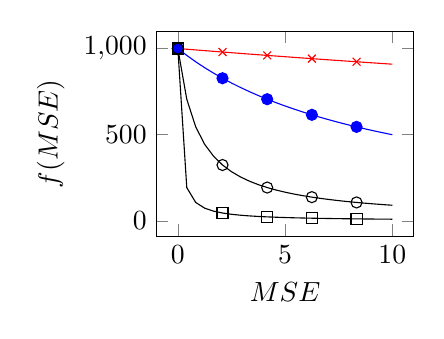
\begin{tikzpicture}[domain=0:10]
    \begin{axis}[xlabel={$MSE$}, ylabel={$f(MSE)$}, width=0.4\linewidth, mark repeat=5, legend entries={{$k=0.01$},{$k=0.1$},{$k=1.0$},{$k=10.0$}}, legend to name=legend_local_refkz, legend columns=4]
      \addplot[mark=x,red]{1000 / (1 + 0.01 * x)};
      \addplot[mark=*,blue]{1000 / (1 + 0.1 * x)};
      \addplot[mark=o,black]{1000 / (1 + 1.0 * x)};
      \addplot[mark=square,black]{1000 / (1 + 10.0 * x)};
    \end{axis}
  \end{tikzpicture}
  \\
  \ref{legend_local_refkz}
  \caption{Графики функции фитнеса для различных значений $k$}
  \label{img:kz}
\end{figure}

\input{cmp_mse_k}

В результате экспериментов по символьной регрессии различных наборов данных было выявлено оптимальное значение коэффициента давления отбора~$k=10.0$. Как видно, данная величина отличается от значения, принятого в исходном алгоритме ПЭГ, следовательно, применение данной модификации можно считать успешным.

%--------------------------------------------------------------------

\subsubsection{Частичный подсчёт фитнеса}

Главным недостатком как эволюционных алгоритмов в целом, так и ПЭГ в частности~--- это их низкая скорость работы (по сравнению со скоростью посторения ИНН, регрессионных моделей)~\cite{ferreira:2001:wsc6Aa}. Любое ускорение алгоритма ПЭГ позволяет улучшить качество получаемых моделей по причине возможности произвести расчёт б\'{о}льшего количества поколений и выполнить больше независимых запусков за эквивалентное время.

Наиболее ресурсоёмкой частью алгоритма является вычисление фитнеса: на вход модели подаются все точки входных данных, которые затем обрабатываются в соответствии с программой (формулой, правилом), закодированной моделью. В ходе исследований, направленных на ускорение процедуры расчёта фитнеса, удалось получить универсальный метод~\cite{SergMir_11_2013_info_problem}, позволивший значительно улучшить оба показателя эффективности: как~$e_{b}$, так и~$r_{f}$.

В формулу расчёта фитнеса как правило входит СКО модели, а само значение фитнеса служит для сравнения эффективности моделей между собой. Было обнаружено, что для такой оценки не требуется вычисление СКО по полному набору подаваемых на вход данных. Если на определённом этапе текущее значение СКО (либо соответствующий фитнес) превысит некоторый порог~$threshold$~--- дальнейшие расчёты могут быть прерваны. Такой подход позволяет избежать лишних затрат на точное вычисление фитнеса плохо приспособленных особей, заменяя его приближённым оценочным значением.

Весь набор входных данных~$DataIn$ перемешивается для избежания последовательностей соседних точек, и разбивается на $G$~пакетов~$Dg_{k}$:

\begin{equation}
\label{eq:zerg_partial_mse_groups}
DataIn=\bigcup_{j=1\ldots G}{Dg_{j}}
\end{equation}

После обработки каждого пакета производится оценка фитнеса, и на её основании выносится решение о прерывании вычислений особи. Условием прерывания служит сравнение фитнеса по вычисленным первым~$K$ группам с пороговым значением~$threshold$, которое динамически изменяется в процессе эволюции и потому задаётся некоторой долей (например,~0.7) от среднего фитнеса популяции на предыдущем поколении:

\begin{equation}
\label{eq:zerg_partial_mse_fit_form}
f(i, g + 1) = f_{z}(i, 0.7 \frac{1}{N}\sum\limits_{j=1}^{N}{f(j,g)})
\end{equation}

\begin{equation}
\label{eq:zerg_partial_mse_fit_form_exp}
f_{p}(i, K) = f_{MSE}(i, \bigcup_{j=1\ldots K}{Dg_{j}}), K \le G
\end{equation}

где $f(i, g + 1)$, $f(i, g)$~--- возвращаемое значение фитнеса~$i$-той особи расчитываемого и предыдущего поколений, $f_{z}(i, threshold)$~--- функция взвешенного фитнеса, $N$~--- размер популяции, $K$~--- количество обработанных групп входных данных. Для того, чтобы внести различие между особями, расчёт которых был прерван в различные моменты времени (пороговое значение ошибки было превышено при разном количестве обработанных групп входных данных), был добавлен коэффициент штрафа~$K/G$:

\begin{equation}
\label{eq:zerg_partial_mse_fitness}
f_{z}(i, threshold) =
	\begin{cases}
		f_{p}(i, G) & f_{p}(i, G) \ge threshold \\
		f_{p}(i, K)\frac{K}{G} & f_{p}(i, K) < threshold
	\end{cases}
\end{equation}

Таким образом, плохие решения будут занимать меньшее количество ресурсов, в то время как лучшие особи будут вычислены наиболее точно. В таблице~\ref{tbl:cmp_fitnesses} приведено сравнение производительности исходных алгоритмов с модифицированными частичным подсчётом СКО.

\input{cmp_fitnesses}




%--------------------------------------------------------------------



\subsection{Выводы}

Какие-то выводы
